\chapter{Introduction to Egress and Ingress Scenarios in Selected CNI Plugins}
\label{cha:introScenarios}
Egress and no egress TODO

\section{Egress Scenario: Routing Outgoing Traffic via Egress Gateway}
\label{sec:egress}

Egress gateway can play key role in cluster's security. It is able to force routing all outgoing connections initiated within labeled pods through gateway node. The node can push all outgoing traffic through a firewall to scan every packet for potential threats, ensuring that outgoing traffic only accesses secure services outside the cluster.

The IT departament of a financial company manages Kubernetes cluster in their local laboratory. The infrastructure is used to create production-ready, efficient and secure environment financial services where handling sensitive data and strict regulatory standards are critical. Leaving unmonitored critical traffic leaving the cluster can create vulnerabilities potentially exposing the system to data exfiltration from financial apps. They decided to analyze all outgoing traffic from financial services pods using some intrusion detection system (IDS) software. However they are also providing some services which do not need such a robust security. Redirecting every request to the traffic analyzer would add unnecessary overhead to exposed applications and cause higher latency. Cluster operators decided to get advantage of an egress gateway routing all outgoing traffic from financial services into security tool to monitor and analyze packets. However end users started complaining about that, their apps started showing errors like "503 Service Unavailable". IT departament administrators started seeking for a problem and they conclude that created egress gateway is a bottleneck in their cluster. They started searching online for solutions and decided to create separate gateways for each deployment of their service \cite{CalicoEgressDeploy}. End users stopped complaining about poor avalaibility of services.

\subsection{Egress Gateway in Selected CNI Plugins}
\label{subsection:egressGateway}

Container Network Interface (CNI) plugins implement own egress gateways offering unique features. This section explores their capabilities in Antrea and Cilium CNI plugins, focusing on how they handle outbound traffic, integrate with other networking components. Understanding these implementations is essential for Kubernetes operators to select the right CNI plugin for their specific requirements.


\subsubsection{Antrea}
\label{subsection:antreaEgress}

Antrea Egress CRD (Custom Resource Definition) API is resource that controls how Pods in a cluster access external services. The resource specifies what egress IP use to selected pods. When a Pod communicates with an external network, the traffic is routed through the Node that has specified egress IP (egress gateway). The source IP address of traffic will then translated to the configured IP address \cite{AntreaEgressArch}.

\begin{figure}[tbh]
    \centering
    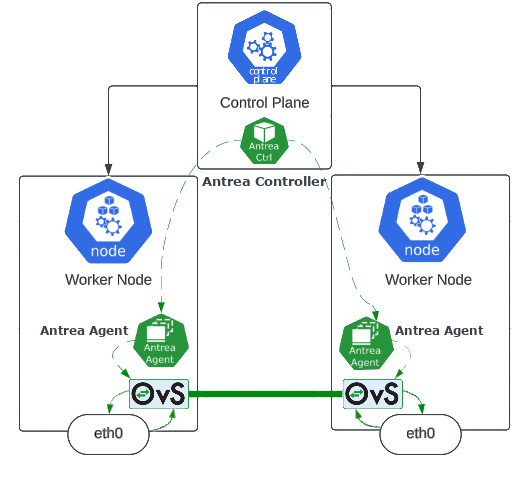
\includegraphics[width=0.6\columnwidth]{images/antrea_overview.png}
    \caption{Antrea Egress Architecture \cite{AntreaEgressArch}}
    \label{fig:antreaEgressArch}
\end{figure}


Figure~\ref{fig:antreaEgressArch} shows architecture of communication flow when configured egress gateway in Antrea CNI. When a pod running on K8s Node tries to access external service (assume is labeled to route its outbound traffic through egress node), the traffic is tunnelled to gateway node and Antrea Agent is performing SNAT. After translation, the next network peer that is comuunicating with egress gateway sees its IP as a source IP instead of IP address of a pod \cite{AntreaEgressArch} \cite{AntreaSNAT}. 

Lets explain egress configuration yaml from Listing~\ref{lst:yamlAntreaEgress} \cite{AntreaEgressArch}:
\begin{itemize}
    \item Antrea allows matching the pods that route through the egress gateway based on two criteria:

    \begin{enumerate}
        \item namespaceSelector -- specifies which pods within the specified namespace should redirect outbound traffic.
        \item podSelector -- selects pods with the specified labels. For example, it can match pods labeled with role: web to redirect traffic.
    \end{enumerate}

    \item egressIP -- specifies SNAT IP address of an egress gateway, to which traffic is tunnelled
    \item externalIPPool -- name of externalIPPool resource which contains pool of IP addresses to allocate if egressIP is not set
\end{itemize}

It is possible to configure fail-over egress gateway node using Antrea implementation. To do that egressIP and externalIPPool must be set (egressIP is in externalIPPool) and when current egress gateway stops working, another node within externalIPPool will be selected. This infrastructure, with a failover service, is part of a high availability setup for production envirnoments (useful for earlier mentioned IT departament) \cite{AntreaEgressArch}.


\begin{listing}[htb]
    \centering
    \caption{Egress resource example \cite{AntreaEgressArch}.}
    \begin{minted}[gobble=4, frame=single, linenos, fontsize=\scriptsize]{yaml}
    apiVersion: crd.antrea.io/v1alpha2
    kind: Egress
    metadata:
        name: egress-prod-web
    spec:
        appliedTo:
        namespaceSelector:
            matchLabels:
            env: prod
        podSelector:
            matchLabels:
            role: web
        egressIP: 10.10.0.8
        externalIPPool: prod-external-ip-pool
    status:
        egressNode: node01
    \end{minted}
    \label{lst:yamlAntreaEgress}
\end{listing}

The ExternalIPPool resource from Listing~\ref{lst:yamlAntreaExternalIPPool} can be configured with the following fields \cite{AntreaEgressArch}:

\begin{itemize}
    \item ipRanges -- IP pools range can be configured using pair of IP (start and end), or by setting cidr (Classless Inter-Domain Routing) range
    \item nodeSelector -- will apply only on nodes specified by this field, e.g. nodes labeled with network-role: egress-gateway
\end{itemize}

\begin{listing}[htb]
    \centering
    \caption{ExternalIPPool resource example \cite{AntreaEgressArch}.}
    \begin{minted}[gobble=4, frame=single, linenos, fontsize=\scriptsize]{yaml}
    apiVersion: crd.antrea.io/v1alpha2
    kind: ExternalIPPool
    metadata:
        name: prod-external-ip-pool
    spec:
        ipRanges:
            - start: 10.10.0.2
              end: 10.10.0.10
            - cidr: 10.10.1.0/28
        nodeSelector:
        matchLabels:
            network-role: egress-gateway
    \end{minted}
    \label{lst:yamlAntreaExternalIPPool}
\end{listing}
  


\subsubsection{Cilium}
\label{subsection:ciliumEgress}

To get advantage of cilium egress gateway features, eBPF masquerading must be enabled and node's kube-proxy component replaced with cilium implementation \cite{CiliumEgressGateway}. Some environments may not be suitable because Cilium requires a kernel version of 5.4 or higher \cite{CiliumInstall}. As shown in Figure~\ref{fig:ciliumEgressArch}, the Cilium agent injects routing information into eBPF maps within the kernel (relying on kernel support for eBPF features). These routes, defined by Cilium policies configured in the control plane, ensure that every node is aware of which pods should redirect traffic to the designated egress node \cite{CiliumEgressGateway}.

\begin{figure}[tbh]
    \centering
    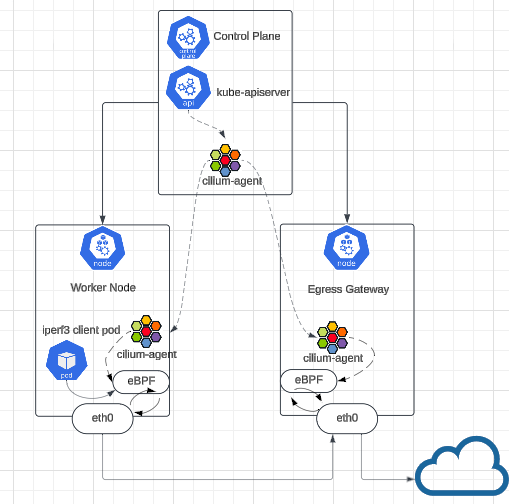
\includegraphics[width=0.9\columnwidth]{images/cilium_egress.png}
    \caption{Cilium Egress Architecture \cite{CiliumEgressGatewayBlog}}
    \label{fig:ciliumEgressArch}
\end{figure}

Simmilian to antrea egress resources, cilium has its own CiliumEgressGatewayPolicy present on Listing~\ref{lst:yamlCiliumEgressGatewayPolicy} \cite{CiliumEgressGateway}:

Cilium allows matching the traffic that route through the egress gateway by \cite{CiliumEgressGateway}:
\begin{itemize}
    \item podSelector -- matching pods based of used selecter, like previous matching labels in antrea, or by matching expressions (key operator, values). More than one podSelector can be used
    \item destinationCIDRs -- an app in pod is requesting some external service, if this resource is match by defined CIDR, the request is routed to egress gateway. For 0.0.0.0/0 all traffic is outgoing by egress gateway. Setting excludedCIDRs is possible to exclude some IPs.
\end{itemize}

Selecting an egress gateway can be done in in three ways: by matching node labels, using IP address in egressIP field (as in antrea) or by interface name. 

\begin{listing}[htb]
    \centering
    \caption{Egress resource example \cite{AntreaEgressArch}.}
    \begin{minted}[gobble=4, frame=single, linenos, fontsize=\scriptsize]{yaml}
    apiVersion: cilium.io/v2
    kind: CiliumEgressGatewayPolicy
    metadata:
    name: egress-sample
    spec:
    selectors:
    - podSelector:
        matchLabels:
            org: empire
            class: mediabot
            io.kubernetes.pod.namespace: default
        matchExpressions:
            - {key: testKey, operator: In, values: [testVal]}
            - {key: testKey2, operator: NotIn, values: [testVal2]}
    destinationCIDRs:
    - "0.0.0.0/0"
    excludedCIDRs:
    - "192.168.1.0/24"
    egressGateway:
        nodeSelector:
        matchLabels:
            node.kubernetes.io/name: a-specific-node
        egressIP: 10.168.60.100
    \end{minted}
    \label{lst:yamlCiliumEgressGatewayPolicy}
\end{listing}


Both Anrea and Cilium allows to configure egress gateway in multiple ways. Cilium has more flexibility in defining which traffic should be routed through egress gateway, unlike Antrea it can specify trafic by destination CIDR. Although cilium has more capabilities of matching egress traffic, antrea implementation allows to create fail-over node, which will route traffic if main one fails. Cilium also takes advantage by using eBPF which is designed for large-scale clusters \cite{CiliumOverview}. It is not clear which egress gateway CNI implementation use, every of them has its advantages and drawbacks. Further both gateways will be evaluated using networking tools in creating local environment.




\section{Ingress Scenario: Splitting Incoming Traffic via Gateway API}
\label{sec:ingress}

The Gateway API as a successor to the Ingress object, provides more features for traffic management and role-oriented approach to separate Kubernetes user/operator concerns. It is capable of teraffic splitting, header modification, or URL rewriting. The Gateway API supports key protocols, like HTTP, HTTPS, TCP, UDP and gRPC. Offering wide range of features, can be used in some different ways \cite{CiliumGatewayAPIBlog}.

%---------------------------------------------------------------------------
\subsubsection{Canary Deployment}
\label{subsubsection:canary}

Canary Deployment is a one of most common deployment methods used to rollout a new application version to end users, ensuring that everything is working as expected before full release. The whole point is to release new version of software only for small group of peoples, leaving most of users unaware of new releas \cite{Canary}.

This is where traffic splitting feature from Gateway API might be used \cite{CiliumTrafficSplitting}. Lets define five stages of deployment \cite{Canary}:

\begin{itemize}
    \item initial state of app -- stable version of application is served
    \item canary stage -- new version of application is only visible for 5\% of users. As some users are able to interact with new provisioned software, most common errors should be visible (if any exist).
    \item early stage -- second stage of canary deployment where new app is available for 25\% of total connections. At this point less frequent bugs might be observed.
    \item mid stage -- allowing for 50\% of end clients. A half of traffic is routed to new version of app. At this point performance of rolledout software is monitored.
    \item late stage -- most of traffic (75\%) is handled by new version of application. Stage that precedes full release of new software.
    \item full stage -- 100\%, new application version is fully deployed for all users
\end{itemize}

If any anomalies are detected during any stage of the canary deployment, the new application version should be immediately rolled back.

Gateway API is not designed for software deployment, it does not have capabilities of rolling back application in automated way. In presented way of use the gateway is used only for weighted traffic splitting.

%---------------------------------------------------------------------------

\subsubsection{Traffic Mirroring with Gateway API}
\label{subsubsection:mirroring}

A company is offering weather API, not all enpoints are publicly available, some features are secured and paid. Securing these paid interfaces is not as critical as more sensitive and confidential data. Lately company decided to start analyzing incomming trafic on secured enpoints, because they make want to make sure only authorized requests are handled. However the company does not have infrastructure capabilities to analyze all incomming traffic on these enpoints. As their services are HTTP based inside Kuberentes cluster, they can get advantage of the Gateway API traffic splitting. The security team decided to route 40\% of incoming traffic to a traffic analyzer to evaluate if and how requests might bypass the paywall. Cluster management (infrastructure providers and cluster operators at once in terms of roles in Gateway API model) decided to split traffic using Gateway API, as they need general usege of API Gateway (company offers RESTful APIs). Pure traffic splitting is not a case, because all incomming traffic have to be handled with response. The solution is to split 40\% of traffic to a different Kubernetes service, then mirror traffic to analyzer and route back to the pod containing an app. While cluster managers implement second deployment with mirroring requests to traffic analyzer, app developers created HTTPRoute object with appropriate weights for each of services. Figure~\ref{fig:mirroringImg} show how cluster infrastucture might look in this case.


\begin{figure}[H]
    \centering
    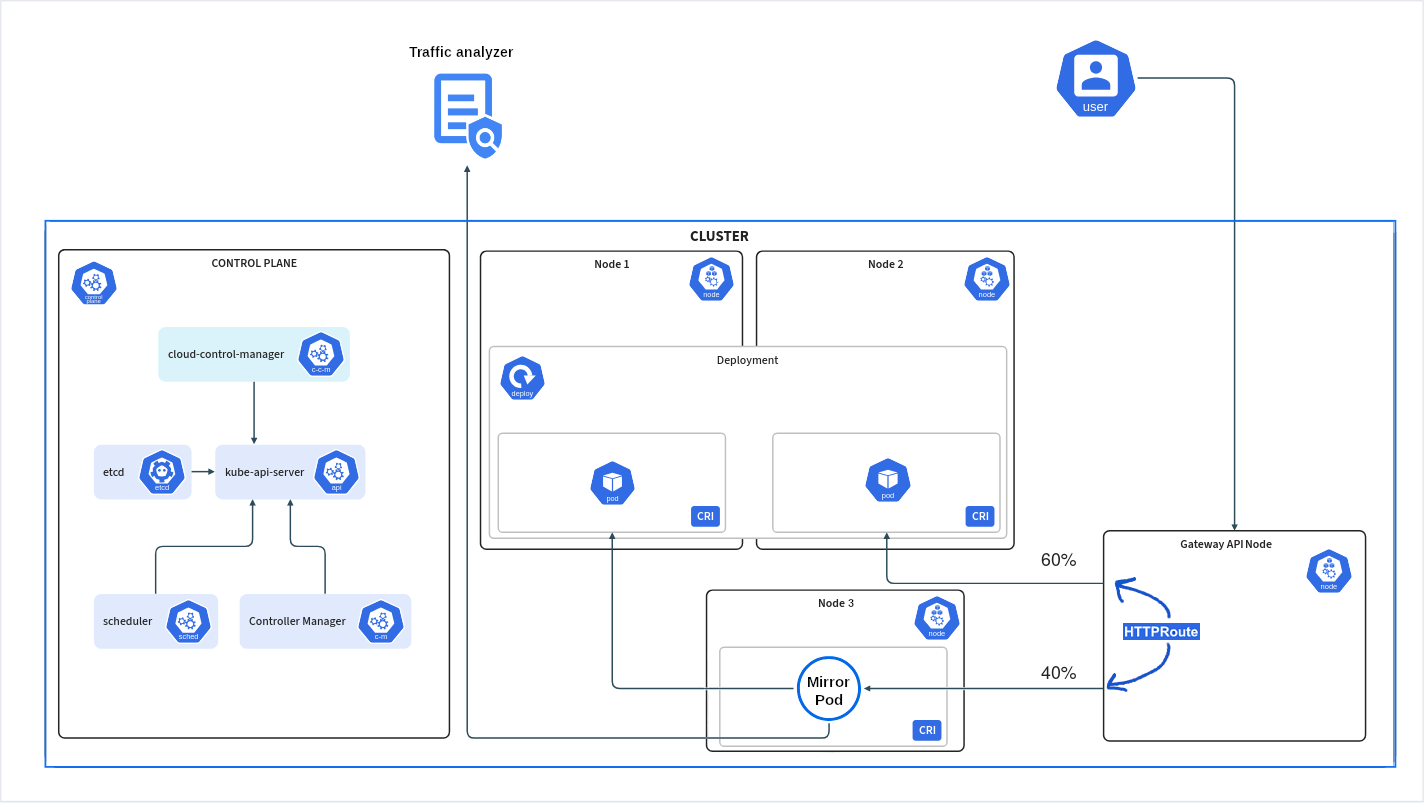
\includegraphics[width=1\columnwidth]{images/ingress.png}
    \caption{Example Kuberenetes cluster with traffic mirroring}
    \label{fig:mirroringImg}
\end{figure}

%---------------------------------------------------------------------------

\subsection{Traffic Splitting in Selected CNI Plugins}
\label{subsection:trafficSplitting}

Unfortunately Antrea plugin does not provide Gateway API implementation, in fact Cilium is the only one which does. For purpose of evaluating cluster networking implementation of Antrea CNI, NGINX Gateway Fabric can be used.



%---------------------------------------------------------------------------
\subsubsection{Antrea + NGINX}
\label{subsection:antreaIngress}

Figure~\ref{fig:canaryAntreaImg} shows example cluster which configures Gateway API to work in canary stage. Antrea CNI is installed, antrea-ctrl and antrea-agent pods are deployed on nodes, OvS tunelling among nodes is set up. On control plane node there is also NGINX Gateway API deployed as a pod, what is in different to cilium, where Gateway API will not be running as a pod.

\begin{figure}[H]
    \centering
    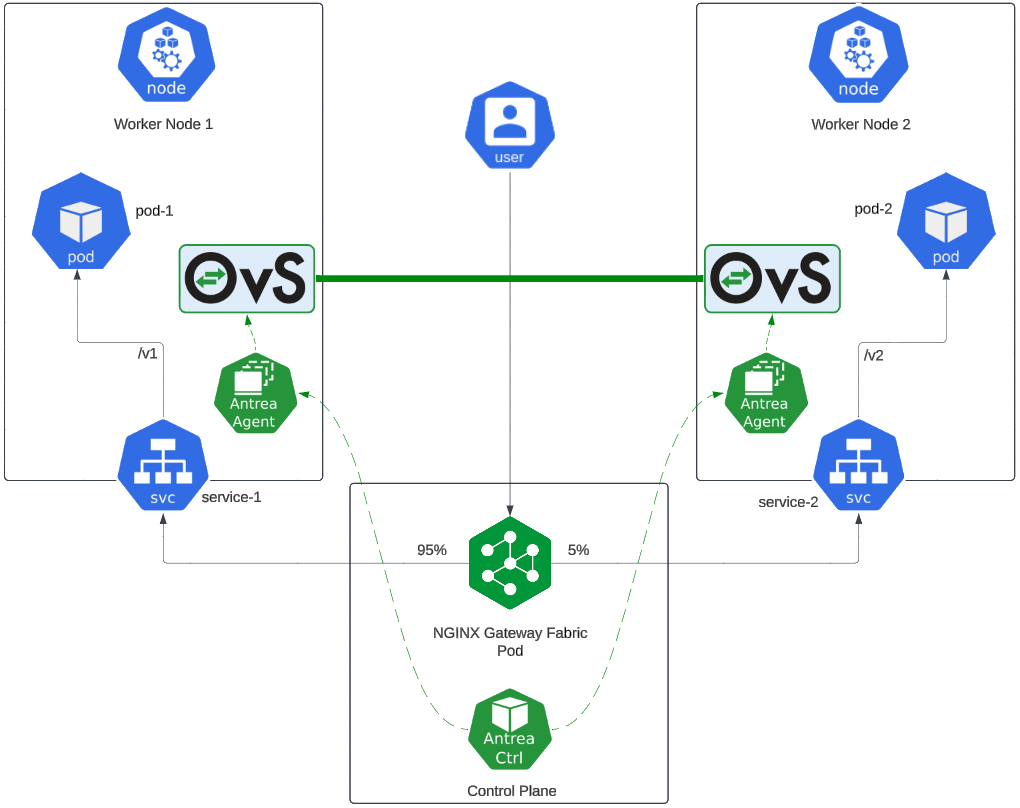
\includegraphics[width=1\columnwidth]{images/antrea-nginx.png}
    \caption{Example Kuberenetes cluster with Antrea CNI and NGINX Gateway Fabric in canary stage of canary deployment}
    \label{fig:canaryAntreaImg}
\end{figure}

\begin{listing}[htb]
    \centering
    \caption{Egress resource example \cite{AntreaEgressArch}.}
    \begin{minted}[gobble=4, frame=single, linenos, fontsize=\scriptsize]{yaml}
    apiVersion: gateway.networking.k8s.io/v1
    kind: HTTPRoute
    metadata:
        name: curren-weather-route
    spec:
        parentRefs:
        - name: nginx-gw
        rules:
        - matches:
            - path:
                type: PathPrefix
                value: /getCurrentWeather
            backendRefs:
            - kind: Service
                name: current-weather-pod-1
                port: 8080
                weight: 95
            - kind: Service
                name: current-weather-pod-2
                port: 8090
                weight: 5
    \end{minted}
    \label{lst:yamlAntreaIngressCanaryHTTPRoute}
\end{listing}
%---------------------------------------------------------------------------
%---------------------------------------------------------------------------
\subsubsection{Cilium}
\label{subsection:ciliumIngress}

%---------------------------------------------------------------------------